\documentclass[smallcondensed]{svjour3}

\usepackage{graphicx}
\usepackage{amsmath,amssymb}
\usepackage{algorithm}
\usepackage{algorithmic}
\usepackage{psfrag}
\usepackage{natbib}

% Better references, I think
\renewcommand{\sec}[1]{Section~\ref{sec:#1}}
\newcommand{\fig}[1]{Figure~\ref{fig:#1}}
\newcommand{\alg}[1]{Algorithm~\ref{alg:#1}}

% Algorithmic changes
\renewcommand{\algorithmicforall}{\textbf{for each}}

%% PSO Stuff
\DeclareMathOperator*{\argmin}{arg\;min}
\DeclareMathOperator*{\argmax}{arg\;max}
\DeclareMathOperator*{\arginf}{arg\;inf}
\DeclareMathOperator*{\argsup}{arg\;sup}
\providecommand{\pers}{\ensuremath{P}}
\providecommand{\neigh}{\ensuremath{N}}
\providecommand{\leftind}{\ensuremath{L}}
\providecommand{\rightind}{\ensuremath{R}}
\providecommand{\nURand}{\ensuremath{U^\neigh}}
\providecommand{\pURand}{\ensuremath{U^\pers}}
\providecommand{\ppos}{\ensuremath{\Vec{x}}}
\providecommand{\fppos}{\ensuremath{\Vec{fx}}}
\providecommand{\pvel}{\ensuremath{\Vec{v}}}
\providecommand{\nbest}{\ensuremath{\Vec{b}^\neigh}}
\providecommand{\fnbest}{\ensuremath{\Vec{fb}^\neigh}}
\providecommand{\pbest}{\ensuremath{\Vec{b}^\pers}}
\providecommand{\fpbest}{\ensuremath{\Vec{fb}^\pers}}
\providecommand{\constriction}{\ensuremath{\chi}}
\providecommand{\ncoeff}{\ensuremath{\phi^\neigh}}
\providecommand{\pcoeff}{\ensuremath{\phi^\pers}}
\providecommand{\obs}{\ensuremath{\Vec{\xi}}}
\providecommand{\ofunc}{\ensuremath{f}}
\providecommand{\swarm}{\ensuremath{swarm}}

%SpecExPSO Stuff
\providecommand{\indic}{\ensuremath{I}}
\providecommand{\specvel}{\ensuremath{\vec{V}}}
\providecommand{\specpos}{\ensuremath{\vec{X}}}
\providecommand{\leftn}{\ensuremath{\Vec{x}^\leftind}}
\providecommand{\rightn}{\ensuremath{\Vec{x}^\rightind}}
\providecommand{\caseset}{\ensuremath{\mathcal{C}}}
\providecommand{\casegen}{\ensuremath{c}}
\providecommand{\casedef}{\ensuremath{(\pbest,\nbest)}}
\providecommand{\casexn}{\ensuremath{(S,-)}}
\providecommand{\casexx}{\ensuremath{(S,S)}}
\providecommand{\casexl}{\ensuremath{(S,\leftind)}}
\providecommand{\casexr}{\ensuremath{(S,\rightind)}}
\providecommand{\casepn}{\ensuremath{(-,-)}}
\providecommand{\casepl}{\ensuremath{(-,\leftind)}}
\providecommand{\casepr}{\ensuremath{(-,\rightind)}}
\providecommand{\casepN}{\ensuremath{(-,N)}}
\providecommand{\casexN}{\ensuremath{(S,N)}}
\providecommand{\noeval}[1]{\ensuremath{#1^{-e}}}
\providecommand{\nonbest}[1]{\ensuremath{#1^{-n}}}
\providecommand{\p}{\ensuremath{p}}
\providecommand{\pset}{\ensuremath{\mathbf{p}}}
\providecommand{\s}{\ensuremath{s}}
\providecommand{\sset}{\ensuremath{\mathbf{s}}}
\providecommand{\nsset}{\ensuremath{\mathbf{ns}}}
\providecommand{\n}{\ensuremath{n}}
\providecommand{\nset}{\ensuremath{\mathbf{n}}}
\providecommand{\nnset}{\ensuremath{\mathbf{nn}}}

%Other math
\providecommand{\prob}{\ensuremath{\mathrm{Pr}}}

\title{A Speculative Approach to Parallelization in Particle Swarm
Optimization}


\date{Received: date / Accepted: date}

\author{Matthew Gardner, Andrew McNabb, and Kevin Seppi}

\institute{M. Gardner \at
Brigham Young University.
3342 TMCB, Provo, UT 84604
Tel.: 801-422-8717
Fax: 801-422-0169
\email{mjg82@byu.edu}
\and
A. McNabb \at
Brigham Young University.
3342 TMCB, Provo, UT 84604
\email{a@cs.byu.edu}
\and
K. Seppi \at
Brigham Young University.
3330 TMCB, Provo, UT 84604
\email{k@cs.byu.edu}
}

\begin{document}
\maketitle

\begin{abstract}

Particle swarm optimization (PSO) has previously been parallelized primarily by
distributing the computation corresponding to particles across multiple
processors.  In these approaches, additional processors can only add more
particles to the swarm.  However, in many cases this is not efficient when
scaled to very large swarm sizes (on very large clusters).  Current methods
cannot answer well the question, ``What do you do with 1000 processors when 50
or 100 particles is the most efficient swarm size?''  In this paper we attempt
to answer that question with a speculative approach to the parallelization of
PSO motivated by speculative execution in modern computer hardware.

In our approach, we refactor PSO such that the computation needed for iteration
$t+1$ can be done in parallel with the computation needed for iteration $t$.
Thus we can perform two iterations of PSO at once.  Even with some amount of
wasted computation, we show that this approach to parallelization in PSO often
outperforms the na\"ive parallelization of simply adding particles to the
swarm.  Our methods produce results that are exactly equivalent to PSO; this is
not a new algorithm or variant, only a new method of parallelization.

However, given this new parallelization model we can relax the requirement of
exactly reproducing PSO in an attempt to produce better results.  We present
several such relaxations, including keeping the best speculative position
evaluated instead of the one corresponding to PSO, and speculating several
iterations ahead instead of just one.  We show that these methods dramatically
improve the performance of parallel PSO in many cases.

\keywords{Parallel algorithms \and Optimization methods \and Particle swarm
optimization \and Speculative Decomposition}

\end{abstract}


\section{Introduction}
\label{sec:intro}

Particle swarm optimization (PSO) has been found to be a highly robust and
effective algorithm for solving many types of optimization
problems~\citep{poli-2008-pso-applications}.  For much of the algorithm's
history, PSO was run serially on a single machine.  However, the world's
computing power is increasingly coming from large clusters of processors.  In
order to efficiently utilize these resources for computationally intensive
problems, PSO needs to run in parallel.

Within the last few years, researchers have begun to recognize the need to
develop parallel implementations of PSO, publishing many papers on the subject.
The methods they have used include various synchronous algorithms
\citep{chu-2006-intelligent-parallel-pso,jin-2005-pso-antenna-designs,%
parsopoulos-2004-parallel-vector-evaluated-pso,%
schutte-2004-parallel-global-optimization-with-pso} and asynchronous algorithms
\citep{mostaghim-2006-multi-objective-pso-on-grids,%
venter-2005-parallel-pso-asynchronous-evaluations}.  Parallelizing the
evaluation of the objective function can also be done in some cases, though
that is not an adaption of the PSO algorithm itself and thus is not the focus
of this paper.

These previous parallel techniques distribute the computation needed by the
particles in the swarm over the available processors.  If more processors are
available, these techniques increase the number of particles in the swarm,
either by adding individual particles or by adding entire new sub-swarms.  In
almost all cases, adding additional particles produces better results in the
same amount of time~\citep{mcnabb-2009-large-particle-swarms}.  In
\fig{iters-sphere} we see an example of this on the well-known benchmark
function Sphere (20 dimensions, reporting the average of twenty runs).  In
terms of the number of iterations performed (which is equivalent to wall-clock
time if all particles are evaluated in parallel), every time the swarm size
increases, the performance improves.

\begin{figure}
  \centering
  \includegraphics[width=.8\columnwidth]{iters_sphere}
  \caption{Function Sphere with various swarm sizes, comparing performance with
  the number of iterations of the algorithm performed.}
  \label{fig:iters-sphere}
\end{figure}

However, it can be seen from the graph that once the swarm is sufficiently
large, doubling the swarm size produces only incremental benefit; performance
improves, but not by very much.  The reason for this is that there comes a
point of diminishing returns with respect to adding particles.  In
\fig{evals-sphere} we show the value obtained after 50,000 function evaluations
(not iterations) as a function of swarm size, again for the function Sphere.
Increasing the swarm size from 5 to 10 has a significant effect on the value
obtained.  However, increasing the swarm size from 16 to 30 makes the algorithm
less efficient; that is, it reduces the progress the algorithm makes per
evaluation.  Other functions show similar trends, though often the optimal
swarm size is slightly larger.  For this reason, previous work has recommended
the use of a swarm size of 50 for
PSO~\citep{bratton-2007-defining-a-standard-for-pso}.  Thus, in at least some
cases, adding particles indefinitely will not yield an efficient
implementation. 

\begin{figure}
  \centering
  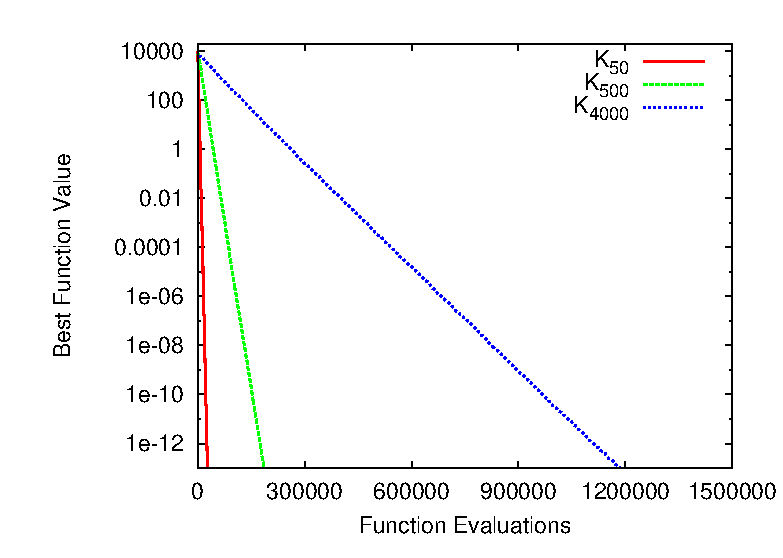
\includegraphics[width=.8\columnwidth]{evals_sphere}
  \caption{Function Sphere with various swarm sizes, comparing performance with
  the number of function evaluations performed.  Error bars show median and
  10th and 90th percentiles.}
  \label{fig:evals-sphere}
\end{figure}

In this paper we consider PSO parallelization strategies for clusters of
hundreds or thousands of processors and functions for which a single evaluation
will take at least tens of seconds, but probably minutes or perhaps hours.  Our
purpose is to explore the question of what to do with a thousand processors
when 50 or 100 particles is the most efficient swarm size, and simply adding
particles results in only incremental improvement.  In our work we assume that
the researcher has some fixed number of processors that should be fully
utilized throughout the optimization process.

In order to solve this problem, we apply the concept of speculative
decomposition~\citep{grama-2003-intro-to-parallel-computing} to particle swarm
optimization, using extra processors to perform two iterations of PSO at the
same time.  Speculative decomposition is analogous to speculative execution
(also known as branch prediction), a technique commonly used in processors.
Modern processors, when faced with a branch on which they must wait (e.g., a
memory cache miss), guess which way the branch will go and start executing,
ensuring that any changes can be undone.  If the processor guesses right,
execution is much farther ahead than if it had idly waited on the memory
reference.  If it guesses wrong, execution restarts where it would have been
anyway.  Thus the processor speculates about future paths of execution in an
attempt to decrease overall processing time.

In this paper we show that the results of standard PSO can be reproduced
\emph{exactly}, two iterations at a time, using a speculative approach adapted
from speculative execution. We prove that the standard PSO equation can be
factored such that a set of speculative positions can be found which will
always include the position computed in the next iteration.  By computing the
value of the objective function for each of the speculative positions at the
same time the algorithm evaluates the objective function for the current
position, it is possible to know the objective function values for both the
current and the next iteration at the same time.  We demonstrate this principle
by implementation and show that it produces exactly the same results as
standard PSO, but two iterations at a time.  The resulting implementation runs
efficiently on large clusters where the number of processors is much larger
than a typical or reasonable number of particles, producing better results in
less ``wall-clock'' time.

It is important to note here that this is not a variant of PSO.  We simply
propose a new way to think about the parallelization of PSO that we show
performs better in many cases than previous parallelizations.

Furthermore, we show that if we relax the requirements of the algorithm, no
longer demanding that it strictly reproduce the exact behavior of standard PSO,
we can introduce new speculative techniques that often out-perform na\"ive
parallelizations of PSO.  These relaxations make better use of the information
obtained from the extra exploration made by the speculative function
evaluations.  We also explore the idea that, like branch prediction in
processors, we need not speculatively evaluate \emph{all} possible future
positions, we can accelerate the algorithm even if we are just \emph{likely} to
have guessed right.  By pruning the speculation to just paths that are
statistically likely to reproduce the paths that are equivalent to PSO we can
increase the swarm size without increasing the number of speculative
evaluations.  We also consider several recovery strategies for cases where the
pruned set of speculative evaluations does not contain the evaluation that
standard PSO would have done.  A further improvement we explore is speculating
several iterations ahead instead of just one, which is made possible by pruning
the number of speculative evaluations.

The balance of this paper is organized as follows. \sec{pso} describes the
particle swarm optimization algorithm, and \sec{related} gives a brief overview
of previous parallelization techniques for this algorithm.  \sec{sepso}
describes mathematically how speculative evaluation can be done in parallel PSO
to perform two iterations at once, then \sec{implementation} gives information
on how to implement this method.  In \sec{relax}, we discuss various methods of
improving the performance of speculative evaluation in PSO, all of which break
the requirement of strictly reproducing the behavior of the original algorithm.
\sec{setup} describes the experiments we ran, and \sec{results} presents the
results of those experiments.  In \sec{conclusion} and \sec{future} we conclude
and discuss future work.

\section{Particle Swarm Optimization}
\label{sec:pso}

Particle swarm optimization was proposed in 1995 by James Kennedy and Russell
Eberhart~\citep{kennedy-1995-particle-swarm-optimization}.  The algorithm is
used to intelligently search a multi-dimensional space by mimicking the
swarming and flocking behavior of birds and other animals. It is a social
algorithm that depends on interaction between particles to quickly and
consistently approximate the optimal solution to a given objective function.

The motion of particles through the search space has three components: an
inertial component that gives particles momentum as they move, a cognitive
component where particles remember the best solution they have found and are
attracted back to that place, and a social component by which particles are
attracted to the best solution that any of their neighbors have found.

At each iteration of constricted PSO, the position $\ppos_t$ and velocity
$\pvel_t$ of each particle are updated as follows:
\begin{align}
\label{eq:velupdate}
	\pvel_{t+1} &=
		\constriction \bigl[ \pvel_t
			+ \pcoeff\pURand_{t}\otimes(\pbest_{t} - \ppos_{t}) +
			\ncoeff\nURand_{t}\otimes(\nbest_{t} - \ppos_{t})
		\bigr] \\
\label{eq:posupdate}
	\ppos_{t+1} &= \ppos_{t} + \pvel_{t+1}
\end{align}
where \( \pURand_{t} \) and \( \nURand_{t} \) are vectors of independent random
numbers drawn from a standard uniform distribution, the \( \otimes \) operator
is an element-wise vector multiplication, $\pbest$ (called personal best) is
the best position the current particle has seen, and $\nbest$ (called
neighborhood best) is the best position the neighbors of the current particle
have seen~\citep{bratton-2007-defining-a-standard-for-pso}.  The parameters \(
\ncoeff \), \( \pcoeff \), and \( \constriction \) are given prescribed values
required to ensure convergence (2.05, 2.05, and .73,
respectively)~\citep{clerc-2002-constricted-pso}. 

Changing the way neighbors are defined, usually called the ``topology,'' has a
significant effect on the performance of the algorithm.  In the Ring topology,
each particle has one neighbor to either side of it; in the Complete
topology\footnote{The Complete topology has often been unfortunately named Star
in the literature, which in graph theory refers to a completely different
topology.  Other names have also been used, including ``global topology'' and
gbest.  We use the graph theory term ``Complete'' in this paper.}, every
particle is a neighbor to every other
particle~\citep{bratton-2007-defining-a-standard-for-pso}.  In all topologies a
particle is also a neighbor to itself in that its own position and value are
considered when updating the particle's neighborhood best, $\nbest$.  Thus with
$p$ particles, using the Ring topology each particle with index $i$ has three
neighbors: $i-1$, $i$ (itself), and $i+1$.  With the Complete topology, each
particle has $p$ neighbors.

In this paper we use these topologies as well as a parallel adaptation of the
Complete topology, called Random, that has been shown to approximate the
behavior of Complete with far less
communication~\citep{mcnabb-2009-large-particle-swarms}.  In the Random
topology, each particle randomly picks two other particles to share information
with at each iteration, along with itself.  Thus in both the Ring and the
Random topologies, all particles have three neighbors.

The ideal topology and swarm size for PSO depend on the objective function.
Researchers have devised various benchmark functions and have found that the
ideal topology for one function may perform very poorly for another function.
The No Free Lunch Theorems for Optimization show that this is true in
general---if an algorithm performs well on average for one class of functions
then it must do poorly on average for other
problems~\citep{wolpert-1997-nfl-for-optimization}.

An attempt to standardize PSO found that although a Complete swarm of 50
particles converged to the global optimum more quickly for many benchmark
functions than the same swarm size with a Ring topology, it was also more
likely to permaturely converge to local optima for other functions.  The study
found no significant improvement for any other swarm size between 20 and 100
and concluded with a recommendation to use a swarm of 50 particles with a Ring
topology as a starting point.  The authors acknowledged that choosing the ideal
topology requires thorough experimentation for the particular
problem~\citep{bratton-2007-defining-a-standard-for-pso}.  Other authors have
explained that a large swarm with a sparse topology propogates information
slowly~\citep{montes-de-oca-2009-frankensteins-pso}.

\section{Related Work}
\label{sec:related}

There have been several parallel implementations of PSO presented in the
literature.  The improvements described in the literature come in two major
areas: innovations in implementation details and innovations in the use of
topology and swarm size to scale PSO to many processors.

\subsection{Innovative Implementations}

There are many ways to parallelize the basic PSO algorithm.  The most
fundamental decision to make in parallel PSO is which parallel architecture to
use.  Several architectures have been proposed, including Master-Slave, fully
distributed (sometimes called ``diffusion''), and reformulating PSO into
Google's MapReduce framework~\citep{belal-2004-parallel-models-for-pso,
mcnabb-2007-parallel-pso-using-mapreduce}.  A somewhat orthogonal
implementation decision when parallelizing PSO is whether to have synchronous
communication or asynchronous communication.

Synchronous parallel implementations of PSO reproduce the standard serial
algorithm exactly.  This approach was first described analytically by
\citet{belal-2004-parallel-models-for-pso} and first implemented by
\citet{schutte-2004-parallel-global-optimization-with-pso}.  In a typical
master-slave algorithm, the master assigns tasks to slave processors, and in
parallel PSO, each task consists primarily of a function evaluation.  Updating
the particle's position and value may also be included in the
task~\citep{belal-2004-parallel-models-for-pso}, or this work may be performed
in serial by the
master~\citep{schutte-2004-parallel-global-optimization-with-pso}.  Before
proceeding to the next iteration, particles communicate, and each particle
updates its neighborhood best.  Whether this communication step happens
sequentially on the master or in parallel, each particle must receive
communication from its neighbors before proceeding.  The benefits of the
synchronous PSO include its simplicity, repeatability, and comparability with
standard PSO, which may be essential in research applications.

Asynchronous parallel
PSO~\citep{venter-2005-parallel-pso-asynchronous-evaluations,
koh-2006-parallel-asynchronous-pso} is a modification to the standard algorithm
which removes the synchronization point at the end of each iteration.  Instead,
particles iterate independently and communicate asynchronously.  In a typical
master-slave implementation of asynchronous parallel PSO, the master updates
each particle's personal best, neighborhood best, velocity, and position
immediately after receiving the function value from the slave processor.  Since
this update occurs while other particles are still being evaluated, it may use
information from the previous iteration for some
neighbors.\footnote{Asynchronous parallel PSO has been compared to the
``asynchronous updates'' variant of serial
PSO~\citep{koh-2006-parallel-asynchronous-pso}.  However, serial PSO with
asynchronous updates differs from standard PSO in that particles use newer
information, but asynchronous parallel PSO differs from standard PSO in that
particles use older information.} In a partially asynchronous implementation,
particles might wait for some but not all neighbors to complete before
proceeding~%
\citep{scriven-2008-asynchronous-pso-in-unreliable-distributed-environments}.
In some master-slave implementations, particles never get more than one
iteration ahead of
others~\citep{venter-2005-parallel-pso-asynchronous-evaluations,
koh-2006-parallel-asynchronous-pso}.  However, in a fully distributed
implementation, particles might never wait for information, and one particle
could complete many more iterations than another
particle~\citep{scriven-2008-distributed-pso-using-peer-to-peer}.  The main
effect of asynchronous evaluation is that processors spend less time
idle---this trait is particularly valuable when processors are heterogeneous or
function evaluation times are
varied~\citep{venter-2005-parallel-pso-asynchronous-evaluations,
koh-2006-parallel-asynchronous-pso}.  Asynchronous parallel PSO behaves
differently than the standard algorithm and may even produce different results
between runs.  Most reports conclude that asynchronous communication produces
similar numerical results to the standard algorithm, but the question has not
yet been thoroughly
addressed~\citep{venter-2005-parallel-pso-asynchronous-evaluations,
koh-2006-parallel-asynchronous-pso}.

\subsection{Scaling PSO to many processors}

The other area of research in parallelizing PSO deals not with the
implementation details of architecture and synchronicity, but with what should
be done with the PSO equations when many hundreds or thousands of processors
are available.  The main issues that have been addressed in this space are how
many particles to use for a particular number of processors and what
communication topology should be employed.

The number of particles per processor has typically been decided by how long it
takes to evaluate the function being optimized.  When the function takes longer
than a few seconds to evaluate, previous techniques have assigned the number of
particles in the swarm to be the number of processors available~%
\citep{jin-2005-pso-antenna-designs,mcnabb-2009-large-particle-swarms},
advocating using as many processors as possible to get the best performance.
When the function takes less time to evaluate than the TCP/IP stack used to
send interprocessor communication, parallel implementations assign several or
many particles to a single processor~\citep{chu-2006-intelligent-parallel-pso,
chang-2005-parallel-pso-with-communication-strategies}.  Often the processor
only sends information about the best particle it evaluated to other
processors~\citep{belal-2004-parallel-models-for-pso}.

Another popular method is simply to run PSO independently on each of the
processors available, taking the best result when all of the runs complete.  It
should be noted that this is equivalent to the previously stated method of
assigning many particles to each processor, only with no communication between
processors instead of little communication.  Both of these methods can be
described as changes in the communication topology of the original PSO
algorithm~\citep{mcnabb-2009-large-particle-swarms}.

Thus previous work in parallelizing PSO, apart from implementation details, has
consisted entirely of increasing the swarm size and adapting the topology to be
better suited to parallel computation.

With regard to increasing the swarm size in PSO, some recent work has suggested
that increasing the swarm size throughout the course of the optimization
process provides better results than having a set swarm
size~\citep{hsieh-2009-efficient-population-utilization-for-pso,
montes-de-oca-2010-incremental-social-learning-pso}.  However, these results
focused on serial computation and are based on total number of function
evaluations, which, when running in parallel on expensive functions, is less
important than total number of iterations.  Other work focusing on
parallelization has shown that when extra processors are available they should
be used, as performance increases with swarm size when measuring in terms of
number of iterations~\citep{mcnabb-2009-large-particle-swarms,
jin-2005-pso-antenna-designs}.  If the swarm size were varied throughout the
course of the optimization process, some processors would be sitting idle at
most iterations.

The contribution of our work is in this area of what should be done with the
PSO equations to better utilize a thousand processors when they are available.
In our work we use a synchronous, MapReduce implementation of parallel PSO.
While we use a specific implementation, we describe how speculative evaluation
can be performed in any of the synchronous architectures mentioned in the
previous section.  The adaptation of our methods to asynchronous PSO
parallelization methods should be straightforward, though it is left to future
work.

\section{Speculative Evaluation in PSO}
\label{sec:sepso}

PSO can be trivially parallelized by assigning each particle's computation to
an individual processor.  But as we have seen in \fig{evals-sphere}, for some
functions, and for large numbers of processors, just adding particles reaches a
point of diminishing returns.  That is, adding processors does not help the
algorithm reach any given level of fitness appreciably faster.  Instead of
adding particles we employ a speculative approach that allows us to perform
two iterations at a time.

Our speculative methods require refactoring the PSO equations such that all
possible positions for each particle at iteration $t+1$ can be evaluated in
parallel along with the position of each particle at iteration $t$.  With some
careful bookkeeping, we can then piece together the results of iteration $t+1$
for each particle, thus using extra processors to evaluate two iterations of
the algorithm in the time it takes to evaluate the function once.  As we show
in Sections~\ref{sec:proof} and~\ref{sec:topology}, a wise choice of topology
limits the necessary speculative evaluations to seven per particle.

To see the value of this refactoring, suppose that $1000$ processors are
available, and that the evaluation of the objective function takes one hour.
If we only want a swarm of $100$ particles, $900$ of the processors would be
sitting idle for an hour at every iteration, and it would take two hours to run
two iterations.  If instead we perform speculative evaluation, sending each of
the $7$ possible speculative positions of a particle to be computed at the same
time as its current position, we would use $800$ of the $1000$ processors and
perform two iterations in one hour.

In order to do two iterations at once, we must use 8 times as many processors
as there are particles in the swarm.  If these processors were not performing
speculative evaluation, they might instead be used for function evaluations
needed to support a larger swarm.  This raises the question of whether a swarm
of 100 particles doing twice as many iterations outperforms a swarm of 800
particles.  We show in \sec{results} that in many, though not all, instances, a
smaller swarm performing more iterations does in fact outperform a larger
swarm.

\sec{proof} shows in detail how the PSO equations can be refactored to allow
for speculative evaluation, proving that our methods are correct and that they
exactly reproduce the behavior of the PSO algorithm.  The section also
introduces some notation used later in the paper.  \sec{topology} gives a brief
discussion of how the topology used affects the amount of speculative
computation needed.

\subsection{Refactoring the PSO Equations}
\label{sec:proof}

To perform two iterations at a time we must first refactor PSO such that the
determination of the value of the objective function is separate from the rest
of the computation.  For simplicity, this discussion will describe the case
where PSO is performing function minimization using the Ring topology.  In this
example, each particle has two neighbors, the ``right neighbor'' and ``left
neighbor,'' whose positions are represented as $\rightn$ and $\leftn$
respectively.  Though we will only describe the case of the Ring topology, this
method can easily be extended to arbitrary topologies.

The refactoring hinges on the idea that once the random coefficients
$\pURand_{t}$ and $\nURand_{t}$ are drawn, there are only a few possible new
positions, or updates, for $\nbest$ and $\pbest$.  For the Ring topology there
are 7 possible update cases, identified in Table~\ref{tab:evals}.  We label
each case with an identifier referring to the source of the update: a minus
sign ($-$) represents no update, $L$ represents an update to $\nbest$ coming
from the left neighbor, $R$ represents an update to $\nbest$ coming from the
right neighbor, and $S$ represents an update to either $\pbest$ or $\nbest$
coming from the particle itself.  As an example, $\casexn$ refers to the case
that the particle finds a new personal best, but neither it nor its neighbors
find a position that updated its neighborhood best.  In the equations that
follow, we refer to an unspecified update case as $\casegen$, and to the set of
cases collectively as $\caseset$.

\begin{table}
  \caption{All possible updates for a particle with two neighbors}
  \label{tab:evals}
  \centering
  \begin{tabular}{lcc}
	Identifier&Source of $\pbest$ update&Source of $\nbest$ update\\
	\hline
	\hline
	$\casepn$&No update&No update\\
	\hline
	$\casepl$&No update&Left Neighbor\\
	\hline
	$\casepr$&No update&Right Neighbor\\
	\hline
	$\casexn$&Self&No update\\
	\hline
	$\casexl$&Self&Left Neighbor\\
	\hline
	$\casexr$&Self&Right Neighbor\\
	\hline
	$\casexx$&Self&Self\\
	\hline
  \end{tabular}
\end{table}

In order to incorporate the determination of which case occurs into the
position and velocity update equations, we introduce an indicator function
$\indic_{t+1}^{\casegen}$ for each case $\casegen \in \caseset$.  When
$\casegen$ corresponds to the case actually taken by PSO,
$\indic_{t+1}^{\casegen}$ evaluates to 1; otherwise it evaluates to 0.  We can
then sum over all of the cases, and the indicator function will make all of the
terms drop to zero except for the case that actually occurs.  For example, the
indicator function for the specific case $\casexn$ (which, as is shown in
Table~\ref{tab:evals}, means that the particle's personal best was updated, but
its neighborhood best was not) can be written as follows:

\begin{align}
  \nonumber
	\indic_{t+1}^{\casexn} & (\ofunc ( \ppos_{t} ) ,\ofunc(\leftn_{t}),
	\ofunc(\rightn_{t}) ,\ofunc(\pbest_{t-1}) ,\ofunc(\nbest_{t-1}))= \\
  \label{eq:deficasexn}
	&\begin{cases}
	   1 & \text{if} \ \ofunc(\ppos_{t}) < \ofunc(\pbest_{t-1}) \\
	   &\quad \text{and} \quad \ofunc(\nbest_{t-1}) < \ofunc(\ppos_{t}) \\
	   &\quad \text{and} \quad \ofunc(\nbest_{t-1}) < \ofunc(\leftn_{t}) \\
	   &\quad \text{and} \quad \ofunc(\nbest_{t-1}) < \ofunc(\rightn_{t}) \\
	   0 & \text{otherwise}
	\end{cases}
\end{align}

For each case $\casegen \in \caseset$, there is also a corresponding
velocity update function $\specvel_{t+1}^{\casegen}$.  When the case is
known, the specific values of $\pbest_t$ and $\nbest_t$ may be substituted
directly into~\eqref{eq:velupdate}.  For example, in case $\casexn$,
$\pbest_{t}=\ppos_{t}$, as \pbest was updated by the particle's current
position, and $\nbest_{t}=\nbest_{t-1}$, as $\nbest$ was not updated at
iteration $t$:
\begin{align}
\nonumber
	\specvel_{t+1}^{\casexn} & (\pvel_t, \ppos_{t}, \leftn_{t}, \rightn_{t},
	\pbest_{t-1}, \nbest_{t-1}, \pURand_{t}, \nURand_{t}) \\
\label{eq:defvcasexn}
		&= \constriction \bigl[ \pvel_{t} +
			\pcoeff\pURand_{t}\otimes(\ppos_{t} - \ppos_{t})
			+ \ncoeff\nURand_{t}\otimes(\nbest_{t-1} -
			\ppos_{t}) \bigr]
\end{align}

In the same way we can create notation for the position update function by
substituting into~\eqref{eq:posupdate}.  For compactness, we will drop the
parameters to $\specvel_{t+1}^{\casegen}$ since they can be inferred from the
subscripts.
\begin{align}
\label{eq:defpcasegen}
	\specpos_{t+1}^{\casegen} & (\ppos_{t}, \pvel_{t}, \leftn_{t},
	\rightn_{t} ,\pbest_{t-1} ,\nbest_{t-1}, \pURand_{t}, \nURand_{t})
	= \ppos_{t} + \specvel_{t+1}^{\casegen}
\end{align}

With this notation we can re-write the original PSO velocity
equation~\eqref{eq:velupdate}, introducing our sum over cases with the
indicator functions.  Again, we represent the indicator functions and velocity
functions without the parameters for compactness.  The equation becomes:
\begin{align}
\nonumber
	\pvel_{t+1} &=
		\constriction \bigl[ \pvel_t
			+ \pcoeff\pURand_{t}\otimes(\pbest_{t} - \ppos_{t})
			+ \ncoeff\nURand_{t}\otimes(\nbest_{t} -
			\ppos_{t}) \bigr] \\
\nonumber
	&= \sum_{c \in \caseset} \indic_{t+1}^{c} \ \constriction \bigl[ \pvel_t
			+ \pcoeff\pURand_{t}\otimes(\pbest_{t} - \ppos_{t})
			+ \ncoeff\nURand_{t}\otimes(\nbest_{t} -
			\ppos_{t}) \bigr]  \\
\label{eq:vel2update}
	&= \sum_{c \in \caseset} \ \indic_{t+1}^{c} \ \specvel_{t+1}^{c} 
\end{align}

Similarly, the position update equation~\eqref{eq:posupdate} becomes:
\begin{align}
\label{eq:pos2update}
	\ppos_{t+1} &= \ppos_{t} + \pvel_{t+1}
	= \sum_{c \in \caseset} \ \indic_{t+1}^{c} \ \specpos_{t+1}^{c} 
\end{align}

The value of the objective function at $\ppos_{t+1}$ is given by:
\begin{align}
\label{eq:val2update}
	\ofunc (\ppos_{t+1}) = \sum_{c \in \caseset} \ \indic_{t+1}^{c}
	\ \ofunc(\specpos_{t+1}^{c})
\end{align}

Returning our attention to the computation of $\ppos_{t+1}$ in
\eqref{eq:pos2update} and writing it with the parameters which were omitted
above, we obtain:
\begin{align}
\nonumber
  \ppos_{t+1} = \sum_{c \in \caseset}
	&\indic_{t+1}^{c}(\ofunc ( \ppos_{t} ) ,\ofunc(\leftn_{t}),
	\ofunc(\rightn_{t}) ,\ofunc(\pbest_{t-1}) ,\ofunc(\nbest_{t-1})) \\
\label{eq:val2updatelong}
	& \specpos_{t+1}^{c}(\ppos_{t},\pvel_{t},\leftn_{t},\rightn_{t},
	\pbest_{t-1},\nbest_{t-1},\pURand_{t}, \nURand_{t})
\end{align}

In this form the important point to notice is that there are only $7$ values
(for this Ring topology) in the set $\{\specpos_{t+1}^{\casegen}: \casegen \in
\caseset\}$ and that none of them depend upon $f(\ppos_t)$ or any other
objective function evaluation at iteration $t$.  Note also that while there are
random numbers in the equation, they are assumed fixed once drawn for any
particular particle at a specific iteration.  Thus PSO has been refactored such
that the algorithm can begin computing all $7$ of the objective function
evaluations potentially needed in iteration $t+1$ \emph{before} $f(\ppos_t)$ is
computed.  Once the evaluation of $f(\ppos_{t})$ is completed for all particles
only one of the indicator functions $\indic_{t+1}^{\casegen}$ will be set to 1;
hence only one of the positions $\specpos_{t+1}^\casegen$ will be kept.

Although this speculative approach computes $\ofunc(\specpos_{t+1}^{\casegen})$
for all $\casegen \in \caseset$, even those for which $\indic_{t+1}^{\casegen}
= 0$, these extra computations will be ignored, and might just as well never
have been computed.  We call the set of computations
$\{\ofunc(\specpos_{t+1}^{c}) : \casegen \in \caseset\}$ ``speculative
children'' because only one of them will be needed.

\subsection{Topology in Speculative Evaluation}
\label{sec:topology}

The number of speculative evaluations needed per particle depends on the number
of neighbors each particle has.  The number of update cases in a topology where
each particle has $n$ neighbors is $2(n+1)$; there are two possibilities for
updates to $\pbest$ (updated by the particle itself and not updated), and $n+1$
possibilities for updates to $\nbest$ (updated by each neighboring particle and
not updated).  When the particle is also a neighbor to itself, as is always the
case in commonly used topologies, one of the cases can be eliminated, as a
particle cannot be the source of an update to its neighborhood best while not
also updating its personal best.  Thus we have $2(n+1)-1$, or $2n+1$,
speculative evaluations per particle.  In a swarm with $p$ particles and $n$
neighbors per particle, $(2n+1)p$ speculative evaluations are needed.

Because the number of speculative evaluations depends on the number of
neighbors a particle has, the choice of topology is an important one.  The use
of the Complete topology, where every particle is a neighbor to every other
particle, would require $O(p^2)$ speculative evaluations per iteration.
Clearly it is much more desirable to have a sparse topology, where $O(np)$ is
much smaller than $O(p^2)$.  However, some functions are better optimized with
the Complete topology and the quick spread of information it entails than with
sparse topologies.  Accordingly, we use the Random topology described
in~\citep{mcnabb-2009-large-particle-swarms}, which has been shown to
effectively simulate the Complete topology.  In~\sec{results} we report the
results for performing speculative evaluation using both the Ring topology and
the Random topology on a number of common benchmark functions.

\section{Implementing Speculative Evaluation}
\label{sec:implementation}

It is not trivial in some parallel architectures to determine which speculative
position was the correct next position of each particle.  In this section we
move from the mathematics of our method to its implementation.  First we
discuss the relatively easy case of a centralized parallel PSO algorithm with a
master computer and many slaves.  In such an architecture, the master keeps
track of all necessary information with only trivial message passing needed.
Then we discuss the more complicated case of a distributed algorithm, where
each particle is on its own and needs to send and receive messages to and from
other particles.  Finally we discuss the further complications of a dynamic
topology, where a particle's neighbors change from one iteration to another.

\subsection{Terminology}

To aid in describing our methodology, we introduce a few terms.  A particle's
set of \emph{speculative children} is the set of all possible next iteration
states (including the particle's position, $\nbest$ and $\pbest$ positions)
that a particle could have.  We use $\p_t$ to denote a particle at iteration
$t$ and $\s_{t+1}$ to denote one of $\p_t$'s speculative children,
corresponding to one of the rows in Table~\ref{tab:evals}.  $\n_t$ is a
neighbor of particle $\p_t$.  Sets of particles are given by $\pset$, $\sset$,
or $\nset$, whereas single particles are simply $\p$, $\s$, or $\n$.

We separate each iteration of PSO into several steps.  First there is the
motion step, where a particle updates its position and velocity.  Then a
particle's position is evaluated, and the particle updates its current value
and its personal best.  Finally, a particle gets information from its neighbors
and updates its neighborhood best.

A particle at iteration $t-1$ that has been moved to iteration $t$ using
\eqref{eq:velupdate}~and~\eqref{eq:posupdate}, but whose position has
not yet been evaluated, is denoted as $\noeval{\p}_t$.  Once its position has
been evaluated, but it has still not yet received information from its
neighbors, it is denoted as $\nonbest{\p}_t$.  Only when the particle has
updated its neighborhood best is it a complete particle at iteration $t$.  It
is then simply denoted as $\p_t$.

\subsection{Centralized Algorithms}

In a centralized, or Master-Slave, parallel PSO algorithm, one machine, the
master, keeps track of all necessary information, and all other machines are
merely used to evaluate the objective function at various positions as directed
by the master~\citep{belal-2004-parallel-models-for-pso}.  To perform
speculative evaluation in such an architecture, the master generates the
positions to evaluate speculatively as in \eqref{eq:defpcasegen}.  After having
the slaves evaluate the objective function at all necessary positions, the
master then decides which position to accept for each particle, as in
\eqref{eq:val2updatelong}.  The outline of the procedure is given in
\alg{centralized}.

\begin{algorithm}
  \caption{Speculative Evaluation in a Centralized PSO}
  \label{alg:centralized}
  \begin{algorithmic}[1]
	\STATE Move all $\p_{t-1}$ to $\noeval{\p}_t$ using
	  \eqref{eq:velupdate}~and~\eqref{eq:posupdate}
	\STATE For each $\noeval{\p}_t$, get its neighbors $\noeval{\nset}_t$ and
	  generate $\noeval{\sset}_{t+1}$ according to
	  \eqref{eq:defpcasegen}.
	\STATE Evaluate all $\noeval{\p}_t$ and $\noeval{\sset}_{t+1}$ in parallel
	\STATE Update personal best for each $\noeval{\p}_t$ and
	  $\noeval{\s}_{t+1}$, creating $\nonbest{\p}_t$ and $\nonbest{\s}_{t+1}$
	\STATE Update neighborhood best for each $\nonbest{\p}_t$, creating
	  $\pset_t$
	\FORALL{$\p_t$}
	\STATE Pick $\nonbest{\s}_{t+1}$ from $\nonbest{\sset}_{t+1}$ that matches
	  the branch taken by $\p_t$ according to
	  \eqref{eq:val2updatelong}.
	\STATE Pass along personal and neighborhood best values obtained by $\p_t$,
	  making $\nonbest{\p}_{t+1}$
	\ENDFOR
	\STATE Update neighborhood best for each $\nonbest{\p}_{t+1}$, creating
	  $\pset_{t+1}$
	\STATE Repeat from Step 1 until finished
  \end{algorithmic}
\end{algorithm}

Given a set of particles at iteration $t-1$ (perhaps which have just been
initialized), the master must move each particle using \eqref{eq:velupdate} and
\eqref{eq:posupdate} to obtain the set $\noeval{\pset}_t$.  For each particle
$\noeval{\p}_t$, the master must then get its set of neighbors
$\noeval{\nset}_t$ and use their positions, along with the position of
$\noeval{\p}_t$, to calculate all possible values of
$\specpos_{t+1}^{\casegen}$, using \eqref{eq:defpcasegen}.  These positions,
along with the original particle's associated information (such as values for
$\pbest$ and $\nbest$), define a set of speculative children,
$\noeval{\sset}_{t+1}$.  The master then has a set of particles
$\noeval{\pset}_t$, and for each particle a set of speculative children
$\noeval{\sset}_{t+1}$, which can all be evaluated at once.

The master then has the slaves evaluate the particles.  Once all particles,
speculative and original, have been evaluated and the values reported to the
master, the master determines which speculative child of each particle was the
correct one.  Mathematically, this corresponds to the evaluation of an
indicator function similar to that found in \eqref{eq:deficasexn}.  In
practice, this is done first by updating each (original) particle's $\pbest$,
if necessary, then by updating the particle's $\nbest$ with information from
the particle's neighbors.  This is simply the original PSO algorithm, and
corresponds to steps 1--5 in \alg{centralized}.  Given the updates to $\pbest$
and $\nbest$, the case from Table~\ref{tab:evals} can be determined, as per
\eqref{eq:val2updatelong}.  The child with the matching case is kept, and all
other speculative children are discarded (step 7 in \alg{centralized}).

The parent $\p_t$ must pass its personal best value to the child, as the child
knows only the position that it guessed, not the function value at that
position.  It is possible that both $\p_t$ and $\s_{t+1}$ update their personal
bests, but $\p_t$'s value is better.  For example, suppose that $\p_{t-1}$ has
a personal best value of 3, and that we are seeking to minimize the function.
$\noeval{\p}_t$ is created, and $\noeval{\s}_{t+1}$ is moved assuming that
$\p_t$ has updated its personal best with its position at time $t$.  Then both
$\noeval{\p}_t$ and $\noeval{\s}_{t+1}$ are evaluated, with values 1 and 2,
respectively.  $\nonbest{\s}_{t+1}$ would think that its current position is
its personal best, as the value it found, 2, is better than its previous
personal best value of 3.  It needs to receive the personal best value from its
parent to know that its personal best position $\pbest$ is actually the
position of $\p_t$, not $\s_{t+1}$.

The parent also needs to pass the value of the neighborhood best that the child
guessed.  The child only knows the position and needs the value in order to
make future comparisons between neighborhood best positions (step 8).

Upon picking the correct branch for each particle and updating the child's
personal best and neighborhood best value (from iteration $t$), the result is
the set $\nonbest{\pset}_{t+1}$, as the particles are now no longer
speculative.  What remains is to update the neighborhood best of those
particles from their neighbors (from iteration $t+1$), as above, to obtain
$\pset_{t+1}$.  That set of particles can subsequently be used to produce the
sets $\noeval{\pset}_{t+2}$ and $\noeval{\sset}_{t+3}$ (steps 1 and 2 in
\alg{centralized}), and the process repeats itself.

\subsection{Distributed Algorithms}

\label{sec:distributed}

In a distributed parallel PSO algorithm, individual processors not only perform
evaluations of particles, but also their movement.  The information for each
particle is not held by a central machine that directs the algorithm; instead,
each processor has the information for the particle or particles that it is in
charge of and must perform the steps of the algorithm for those
particles~\citep{mcnabb-2007-parallel-pso-using-mapreduce}.  Messages such as
values and positions for the neighborhood best are sent between processors.
There may still be some machine that collects information from all of the
particles and outputs the result of the algorithm, though that machine's
importance is much less than in centralized algorithms.

To perform speculative evaluation in a distributed PSO algorithm, there must be
some way to have processors evaluate the speculative children of particles,
without giving the speculative particles the same treatment as actual
particles, as the speculative children only live for one iteration.  One way
that can be done is by assigning each particle a set of machines instead of a
single machine, and the particle directs its extra machines to evaluate its
speculative children.  The same information needs to be passed between
particles no matter the framework used.  We describe here the messages each
particle needs to receive to perform speculative evaluation.

A processor that is controlling a single particle $\p_{t-1}$ must first move
the particle to $\noeval{\p}_t$ and produce the particle's speculative children
$\noeval{\sset}_{t+1}$.  This is done in the same way as described above.
However, in order to produce $\noeval{\sset}_{t+1}$, the processor needs
information about the particle's neighbors, so there must be some message
passing to get that information.  Particularly, the information that the
processor needs is the position of each of the particle's neighbors at
iteration $t$.

To get that information, a round of message passing is required.  Each particle
sends its position to its neighbors at iteration $t$, so that all particles can
generate $\noeval{\sset}_{t+1}$.  After each particle evaluates its position
and the positions of its speculative children, it passes information about the
outcome of iteration $t$ to its neighbors, so that neighboring particles can
update their neighborhood bests to move from $\nonbest{\p}_t$ to $\p_t$.  Once
that communication is finished, the particle can select the speculative child
which matched the branch that iteration $t$ actually produced.  Then another
round of information passing follows, for iteration $t+1$, so that
$\nonbest{\p}_{t+1}$ can be updated to $\p_{t+1}$.  Two iterations have then
been completed with only one round of evaluations, and the next iteration can
start again with the first round of message passing.

In distributed frameworks, synchronizing all of the machines for a round of
message passing can be expensive.  The method just described uses three rounds
of message passing for every two iterations (corresponding to steps 2, 5 and 10
in \alg{centralized}).  It is possible to perform speculative evaluation in PSO
with only one round of communication per two iterations.  However, the
methodology is tedious and is not the focus of this paper, so we defer its
description to the Appendix.

\subsection{Dynamic Topologies}

Performing speculative evaluation in PSO with a dynamic topology (where
neighbors change from iteration to iteration) raises a sticky issue of its own.
In a static topology, at iteration $t$ a particle already has all of the
information about the positions of its neighbors during iterations $1$ through
$t-1$.  If the neighbor finds a better position at iteration $t$, the particle
updates its neighborhood best, but if it does not, it still has its old
neighborhood best from its neighbors for all previous iterations.

In a dynamic topology, a particle might not have information about the previous
positions of its neighbors at iteration $t$.  That means that its new
neighborhood best could come not only from its neighbors' positions at
iteration $t$, but also from their personal best from iteration $t-1$, as
neighbors' personal bests are what are used to update a particle's neighborhood
best.  That creates a problem for speculative evaluation---there are
potentially more than $2n+1$ possible next positions, increasing the amount of
work that must be done to perform the second iteration at the same time as the
first.

This is easily fixed by updating each new particle $\noeval{\p}_{t+2}$ with the
currently available information about its neighbors $\noeval{\nset}_{t+2}$
before producing its children $\noeval{\sset}_{t+3}$.  If a particle
$\noeval{\p}_{t+2}$ updates its neighborhood best with the personal bests of
$\noeval{\nset}_{t+2}$ before calculating the next possible positions for
$\noeval{\sset}_{t+3}$, there are still only $2n+1$ possible next positions,
and the problem is avoided.

\section{Relaxing the Requirements}
\label{sec:relax}

While the idea of speculative evaluation in particle swarm optimization is
intriguing, the results in \sec{results} show that in many cases it requires
too many extra evaluations to produce competitive results.  On most functions,
the larger swarm size that can be used in na\"ive parallelizations leads to
better performance than is found by trying to do speculative evaluation to
exactly reproduce PSO.  However, if we keep the idea of speculative evaluation
while relaxing the requirement of exactly reproducing the behavior of the
original PSO algorithm, we see some impressive results.

We outline three main improvements to speculative evaluation.  First, in
\sec{pickbest} we describe a method that uses all of the information found in
doing speculative evaluations.  Then Sections~\ref{sec:pruning}
through~\ref{sec:wrong} present a technique that reduces the number of
speculative evaluations that need to be done for each particle.  Finally,
\sec{manyiters} shows a method for speculating several iterations ahead,
instead of just one.

None of these methods fundamentally change the PSO algorithm.  They simply lead
to particles having different values for personal and neighborhood best
positions than would have occurred in standard PSO, because they receive
different information.  This kind of relaxation is fairly typical in the
parallelization of PSO~\citep{koh-2006-parallel-asynchronous-pso}.

\subsection{Pick the Best Child}
\label{sec:pickbest}

In performing speculative evaluation as we have described it, $2n+1$
speculative evaluations are done per particle, while all but one of them are
completely ignored.  It seems reasonable to try to make use of the information
obtained through those evaluations instead of ignoring it.

To make better use of the extra speculative evaluations, instead of choosing
the speculative child that matches the branch that the original PSO would have
taken, we take the child that has the best value.  The methodology is exactly
the same as above except for the process of choosing which speculative child to
accept.  The only change needed in \alg{centralized} is in step 7, where
$\noeval{\s}_{t+1}$ with the best value is chosen from $\noeval{\sset}_{t+1}$
instead of with the matching branch.  We call this technique Pick Best.

This can be thought of as drawing a number of samples from the next iteration
and accepting the best one.  Speculative particles that move in good directions
are kept.  Intuition says that this technique favors exploitation over
exploration, but as we will show in \sec{results}, that is not always the case.

At this point it is also interesting to note a parallel between our methods and
parallel evolution
strategies~\citep{rudolph-1991-distributed-evolution-strategies}.  In evolution
strategies, a parent individual (representing a potential solution to some
objective function) produces a number of offspring by a mutation operator.  One
of the individuals is selected by a selection operator, and that individual
becomes the parent for the next
generation~\citep{beyer-2002-evolution-strategies}.  Our methods are similar,
where our mutation operator is simply the PSO motion equations and the
selection operator is either the indicator function introduced in \sec{sepso},
in the case of our original speculative algorithm, or the standard selector
operator based on fitness, in the case of this Pick Best technique.


\subsection{Pruning the Speculative Evaluations}
\label{sec:pruning}

Because the problem facing speculative evaluation is having too many possible
evaluations to perform, a natural step to take is to eliminate some of the
evaluations.  If we could reliably predict which branch were going to be taken,
we could limit ourselves to one speculative evaluation per particle instead of
$2n+1$.  With a fixed number of processors, this would allow us to greatly
increase the swarm size relative to that needed in the original speculative
algorithm (e.g., with 120 processors, a na\"ive parallelization has a swarm of
size 120, complete speculative evaluation has a swarm of size 15, and pruning
the evaluations to only one per particle allows a swarm of size 60).  As not
all of the branches are evaluated in any given iteration, we call this
technique pruning.  

A na\"ive approach to pruning is to keep track of the last branch taken by each
particle and speculate on that branch.  This turns out to be correct far less
than half of the time on average.

A more principled approach would be to use the statistical behavior of PSO to
find probabilities of taking any particular branch.  While we cannot with
certainty predict which branch a particle will take every time, if we can use
statistics to narrow down the $2n+1$ possible evaluations to a few likely
candidates, we can decrease the amount of computation required to do
speculative evaluation and improve our performance.

\subsection{Branch Statistics}
\label{sec:statistics}

In Table~\ref{tab:evals} we presented all possible branches that a particle
with two neighbors could take.  Here we lump all of the neighbors together and
consider the statistics for the five branches shown in
Table~\ref{tab:branches}.  In the identifiers, N represents an update to
$\nbest$ coming from any neighbor.

\begin{table}[ht]
  \caption{Five Branches to Consider for Statistics}
  \label{tab:branches}
  \centering
  \begin{tabular}{lcc}
	Identifier&Source of $\pbest$ update&Source of $\nbest$ update\\
	\hline
	\hline
	$\casepn$&No update&No update\\
	\hline
	$\casexn$&Self&No update\\
	\hline
	$\casexx$&Self&Self\\
	\hline
	$\casepN$&No update&Some Neighbor\\
	\hline
	$\casexN$&Self&Some Neighbor\\
	\hline
  \end{tabular}
\end{table}

\begin{table}[ht]
  \caption{Branch Statistics in PSO}
  \label{tab:stats}
  \centering
  \scriptsize
  \begin{tabular}{c|c|c|c|c|c|c}
	Topology&Function&\casepn&\casexn&\casexx&\casepN&\casexN\\
	\hline
	\hline
	Ring&Sphere&53.0\%&9.3\%&11.4\%&20.2\%&6.2\%\\
	&Griewank&51.7\%&8.4\%&12.2\%&20.7\%&7.0\%\\
	&Rastrigin&49.5\%&4.8\%&14.6\%&21.3\%&9.9\%\\
	&Rosenbrock&51.3\%&7.4\%&12.9\%&21.1\%&7.3\%\\
	\cline{2-7}
	&Average&{51.3\%}&{7.5\%}&{12.8\%}&{20.8\%}&
	{7.6\%}\\
	\hline
	\hline
	Random&Sphere&66.7\%&11.9\%&2.6\%&15.6\%&3.1\%\\
	&Griewank&69.0\%&10.9\%&2.5\%&14.9\%&2.7\%\\
	&Rastrigin&81.9\%&5.5\%&1.5\%&10.0\%&1.0\%\\
	&Rosenbrock&74.2\%&7.7\%&2.2\%&14.0\%&1.8\%\\
	\cline{2-7}
	&Average&{73.0\%}&{9.0\%}&{2.2\%}&{13.6\%}&
	{2.2\%}\\
	\hline
	\hline
	Complete&Sphere&31.9\%&9.2\%&0.2\%&45.1\%&13.5\%\\
	&Griewank&35.3\%&8.4\%&0.2\%&44.1\%&11.9\%\\
	&Rastrigin&47.7\%&6.7\%&0.2\%&38.2\%&7.0\%\\
	&Rosenbrock&35.3\%&3.4\%&0.3\%&54.4\%&6.6\%\\
	\cline{2-7}
	&Average&{37.6\%}&{6.9\%}&{0.2\%}&{45.5\%}&
	{9.8\%}\\
	\hline
  \end{tabular}
\end{table}

Row 1 in Table~\ref{tab:branches}, \casepn, corresponds to the phenomenon
commonly called stagnation in the literature, but with only a single particle.
As an interesting aside, we found that complete stagnation (where the entire
swarm is stagnant) practically never occurs in PSO, though frequently large
percentages of the swarm are stagnant.  Iterations where the entire swarm is
stagnant average less than 2 in 1000 iterations, unless the swarm converges
beyond machine precision.  When graphs of the best function value flat-line,
what really has happened is a contraction of the particles' velocity, not
stagnation in the technical sense.  

We seek to find the probability of taking any given branch, given whatever
information is needed: $\prob(\caseset_t|\cdot)$.  In finding these
probabilities, we do not attempt to derive any distribution from the PSO
equations, we simply look at empirical distributions.  However, even with
empirical distributions, the problem with this approach is that it is not clear
what information influences the probability of taking a branch.  The failure of
the naive approach seems to say that the previous branch, $\caseset_{t-1}$, is
not incredibly useful.  We look at two factors that we believe have a
significant influence on $\prob(\caseset_t)$: topology and function.  Thus we
are looking at $\prob(\caseset_t|T,F)$.

We show in Table~\ref{tab:stats} with what percentage a particle takes each of
these branches for three different topologies and four different functions.
All of our statistics are from swarms of 240 particles.  Brief experimentation
showed that other swarm sizes had similar statistics.  We ran 750 iterations on
all combinations of functions and topologies except for the functions Griewank
and Rastrigin with the Complete topology.  We found that those runs frequently
converged past machine precision after 500 iterations, and that led to
erroneously high values for the probability of stagnation.  Instead we ran for
only 450 iterations on those two combinations.  All of our results were
averaged over 20 runs of the algorithm; thus the probabilities presented are
the averages of 3.6 million trials for the branch taken (2.16 million for the
two with only 450 iterations).  Table~\ref{tab:stats} contains the results.
The definitions for all of the functions in the table are found in \sec{setup}.

The probabilities presented in Table~\ref{tab:stats} are interesting in and of
themselves and could probably be used to better understand the characteristics
of various topologies.  It is notable that there is small variation between
functions in any given topology, but the variation across topologies is far
greater.  However, our concern is with speculative evaluation.  We are
interested in predicting the branch that any given particle will take at a
particular iteration.  For our purposes, it appears that given a topology, the
probability of selecting a branch and the function are close to independent, or
$\prob(\caseset_t|T,F) \approx \prob(\caseset_t|T)$.

From Table~\ref{tab:stats} we can see that with the Random topology, we can
pick the first branch, corresponding to stagnation, and be right around 70\% of
the time.  With the Ring topology, we would be right 50\% of the time.
Branches \casepN\ and \casexN\ really correspond to several actual branches, as
all of the neighbors are lumped together.  The 20\% probability of taking
branch \casepN\ with the Ring topology can be split into two branches, as there
are only two neighbors.  It also turns out that the neighbor that last updated
the neighborhood best is the most likely to update it next time, so keeping
track of that information could be fruitful in trying to predict that branch.

The statistics for the Complete topology are less promising, as there are 240
neighbors that branch \casepN\ splits into, instead of two.  Pruning does,
however, allow for the possibility of using the Complete topology in
speculative evaluation while avoiding the explosion in the number of
evaluations it would otherwise entail.  Though pruning makes its use possible,
we still found the communication costs in our parallel environment prohibitive,
so we do not present any results for the Complete topology here.

With the other topologies, however, there are a few branches with very high
probabilities, so we can have hope that cutting out some of the evaluations
that have low probability will lead to an increase in overall performance.  In
order to implement this kind of pruning, the only change that needs to be made
to \alg{centralized} is in Step 2, where the speculative children are
generated.  Instead of generating all possible speculative children, generate
the subset of the children that is desired.

\subsection{Recovering from Pruning Too Much}
\label{sec:wrong}

When not all of the branches are evaluated, there is some probability of not
evaluating the branch that was actually taken by the original particle.  There
are a few possibilities for recovery in this case.  One is to leave the
particle as it is, not accepting any of the speculative evaluations, because
none of them were correct.  This leads to particles being at different
iterations, as some particles guess correctly while others do not.  Thus we
lose exact compatibility with the original PSO, though this particular
relaxation is nothing new; asynchronous adaptations of PSO do the same
thing~\citep{koh-2006-parallel-asynchronous-pso}.  As an aside, it is equivalent
in this case to simply increment the iteration number of particles which fail
to correctly predict their branch.  This keeps the iteration number constant
across all particles, simplifying the work needed to be done in determining
neighbors when dynamic topologies are involved.  We call this technique Social
Promotion.

Another possibility is to pick the best child, as described in \sec{pickbest}.
This ignores the fact that the branch might have been wrong; it does not
matter, because we simply accept the child that had the best value.  In most of
the experiments that we ran, it turned out that picking the best child
performed better than keeping the particle back an iteration.

\subsection{More than one iteration ahead}
\label{sec:manyiters}

We need not simply produce speculative children for the next iteration.  We can
view all possible speculative evaluations for a particle as an infinite tree
with branching factor $2n+1$.  As we have already seen that doing one full
level of the tree produces too many extra evaluations to be profitable, it is
incredibly unlikely that doing two full iterations would produce decent
results.  But, if the idea of speculating more than one iteration ahead is
combined with wisely pruning the possible evaluations based on branch
statistics, we can use just a few extra evaluations to go two or more
iterations ahead on the most likely branches.

When speculating more than one iteration ahead, the idea of Social Promotion
cannot feasibly be implemented, as we can only determine correct branches for
the first iteration.  Thus in this case we always pick the child that has the
highest value.

The question of which branches to take in this infinite tree is an intriguing
one that we can only begin to explore here.  If the branch corresponding to
stagnation has a 75\% chance of being taken, as in the Random topology with
most functions, we could speculate three iterations ahead on that branch and
still have a 42\% chance of predicting correctly.  However, intuition would say
that perhaps it is better to hope that the particle is productive instead of
stagnant, so a branch where the particle updates its personal best might be
more fruitful to try.  In our experiments we try just one of the countless
possibilities, but one that turns out to work very well.  More work is needed
to compare the different branching possibilities on various functions.

\section{Experimental Setup}
\label{sec:setup}

We ran experiments to compare our speculative parallelization of PSO to the
na\"ive parallelization.  At each iteration of the algorithms, we use one
processor to perform one function evaluation for one particle, be it
speculative or non-speculative.  The speculative version actually performs
two iterations of PSO at each ``iteration,'' so we instead call each
``iteration'' a ``time step.''

Because our interest is in exploring the most efficient use of processors, we
must hold fixed the number of processors used at each time step in all of our
experiments, giving all approaches the same number of function evaluations.
Thus while we label our graphs with ``Time Steps,'' this is equivalent to the
number of function evaluations used by each approach (simply multiply by the
number of processors to transform time steps to function evaluations).  We use
``Time Steps'' to reflect wall-clock time, as our primary interest is using
extra processors in parallel to improve performance on functions with long
evaluation times.  A smaller swarm running serial PSO would likely produce
better results than we present in the same number of function evaluations, but
because the function evaluations were not done in parallel it would take more
wall-clock time.  When comparing the performance of parallelized algorithms on
long-running functions, we must compare by wall-clock time with the same
resources, not solely by the number of function evaluations.

We also do not report absolute time used by each algorithm, as specific time
values are heavily implementation-dependent.  Using time steps, where at every
time step each processor evaluates the function once, is an abstraction from
individual implementations that still conveys all of the information necessary
to compare algorithms.  In this paper we focus on the effects of algorithm
choices on parallel PSO performance.  As there are inexpensive functions with
complex landscapes and expensive functions with simple landscapes, the behavior
of PSO with respect to the function is the main issue.  For this purpose,
benchmark functions are a useful and efficient tool for understanding the
effects of PSO with expensive objective functions even though the benchmark
functions are themselves inexpensive.  For example, a plot of performance with
respect to iterations for a smooth unimodal function with five minutes per
evaluation would be similar to that of Sphere.

Using the same number of processors for each approach requires that our
speculative parallelizations have a smaller swarm size than the na\"ive
parallelization.  For each of the topologies we used, a particle has three
neighbors including itself.  As shown in Table~\ref{tab:evals}, this results in
$7$ speculative evaluations per particle.  With one evaluation needed for the
original, non-speculative particle, we have $8p$ evaluations for every two
iterations, where $p$ is the number of particles in the speculative swarm.  The
extra evaluations required in our speculative approach would instead be used to
evaluate particles in na\"ive parallelizations, so we compare swarms of size
$p$ in speculative evaluation with swarms of size $8p$ in na\"ive approaches.

Where the Complete topology would normally be preferred, we use a Random
topology in our speculative approach, as Complete leads to an explosion in the
number of speculative evaluations.  If speculative evaluation were not being
performed, it is possible that the Complete topology would be used.  However,
the Complete topology also requires a very large amount of interprocessor
communication in distributed PSO, so it is still quite possible that Random
would be used even with na\"ive parallelizations.  But, to be fair in our
comparisons, we compare to the na\"ive parallelization using both the Random
topology and the Complete topology (labeled PSO Random and PSO Complete in our
results).  

We experimented with five common benchmark problems defined
in~\citep{herrera-2010-test-suite}: Rastrigin, Sphere, Schwefel 2.21, Griewank,
and Bohachevsky.  

Rastrigin is initialized in $[-5.12,5.12]^D$ and is defined as:
\[f(\Vec{x}) = \sum_{i=1}^D\left(z_i^2 - 10\cos\left(2\pi z_i\right) +
10\right), z=x-c\]

Sphere is initialized in $[-50,50]^D$ and is defined as:
\[f(\Vec{x}) = \sum_{i=1}^D z_i^2, z=x-c\]

Schwefel 2.21 is initialized in $[-500,500]^D$ and is defined as:
\[f(\Vec{x}) = \max_i{|z_i|, 1 \leq i \leq D}, z=x-c\]

Griewank is initialized in $[-600,600]^D$ and is defined as:
\[f(\Vec{x}) = \frac{1}{4000}\sum_{i=1}^D z_i^2 - \Pi_{i=1}^D
\cos\left(\frac{z_i}{\sqrt{i}} \right) + 1, z=x-c\]

And Bohachevsky is initialized in $[-15,15]^D$ and is defined as:
\[f(\Vec{x}) = \sum_{i=1}^D(x_i^2+2x_{i+1}^2-.3\cos(3\pi x_i)-.4\cos(4\pi
x_{i+1})+.7)\]

In computing the branch statistics in \sec{statistics}, we also used the
Rosenbrock function.  That function is defined as:
\[f(\Vec{x}) = \sum_{i=1}^D \left(100(x_{i+1}-x_i^2)+(x_i-1)^2\right)\]

The $c$ in the function definitions is a shifted center, in order to avoid
origin-seeking bias in the PSO algorithm and its
variants~\citep{monson-2005-origin-seeking-bias}.  We move the center of the
shifted functions (all except Bohachevsky) to be halfway between the center and
the boundary of the initialization region.  For example, if the initialization
region is $[-50,50]^D$, the center is $(25)^D$.  For all of these functions we
used 20 dimensions.

The parallelization techniques we compare are the na\"ive parallelization (here
labeled Na\"ive simply for ease of reference), our original speculative
approach (labeled SEPSO), and the four relaxations of SEPSO discussed in
\sec{relax}.  In presenting our results, we call the approach developed in
\sec{pickbest} Pick Best.  The methods described in \sec{pruning} through
\sec{wrong} are called Pick Best Pruned and Social Promotion Pruned, and the
method in \sec{manyiters} we call Many Iterations.

When performing pruning in Pick Best Pruned and Social Promotion Pruned, there
are a large number of ways to prune speculative evaluations.  We experimented
with several, but present results for only one possible pruning.  The pruning
we present uses only the two branches where the $\nbest$ value was not updated:
\casepn\ and \casexn.  Those branches are convenient in that no messages are
needed from neighbors in order to produce the positions of the speculative
particles---in distributed frameworks using several rounds of communication
(see \sec{distributed}), one of the rounds of communication can be dropped
entirely.

Because pruning only requires two speculative evaluations per particle (along
with evaluating the original particle), we can use swarms of size
$\frac{1}{3}p$ to compare to a swarm of size $p$ with the na\"ive
parallelization, instead of $\frac{1}{8}p$ with other techniques.

There are also many ways to speculate several iterations ahead, and with Many
Iterations we again only show results for one of them.  The combination of
branches we tried uses seven speculative evaluations per particle, matching the
swarm size of the original speculative algorithm.  The seven evaluations we
used corresponded to several iterations of branches \casepn\ and \casexn.  Two
of the evaluations were just one iteration ahead, four were two iterations
ahead, and one was three iterations ahead.  The evaluations that were one
iteration ahead were branches \casepn\ and \casexn; those that went two
iterations ahead were formed by taking either branch \casepn\ or \casexn and
then branch \casepn\ or \casexn; and the evaluation going three iterations
ahead followed branch \casepn\ on all three iterations.


\section{Results}
\label{sec:results}

\subsection{Rastrigin}

First we look at Rastrigin.  Rastrigin is a multi-modal function that is best
optimized with a large, Complete swarm.  It has been shown that with Rastrigin,
the more particles there are in the swarm, the lower function value it finds,
up to at least 4000 particles~\citep{mcnabb-2009-large-particle-swarms}.
Smaller swarms get caught in local optima.  Because our speculative algorithms
require significantly smaller swarm sizes, we would expect to not perform very
well on functions such as Rastrigin.  Our experiments show our intuition to be
correct.  In this experiment we used 240 processors, so SEPSO and Pick Best
each had 30 particles, and the Na\"ive algorithms had 240 particles.  As
expected, SEPSO and Pick Best converge quickly to worse local optima than
Na\"ive does.  \fig{rastrigin} shows the results graphically.

\begin{figure}
  \centering
  \includegraphics[width=.8\columnwidth]{rastrigin}
  \caption{Function Rastrigin with a swarm that uses 240 processors per time
  step.  Recall that at each time step all processors evaluate the function
  once.  All speculative algorithms use the Random topology.}
  \label{fig:rastrigin}
\end{figure}

\subsection{Sphere}

Next we go to Sphere, the simplest of common benchmark functions.  The function
has no local optima (only a single global optimum) and is best optimized in
terms of function evaluations with a small swarm using a Complete topology.  We
expect our methods to be perfect for such functions, and our results show this
intuition again to be correct.  First we compare the basic SEPSO approach to
Na\"ive.  In \fig{basic-sphere} we can see that when both SEPSO and Na\"ive are
using a Random topology, SEPSO clearly outperforms Na\"ive.  However, the
comparison between SEPSO and Na\"ive Complete is not as encouraging---Na\"ive
Complete performs slightly better.

\begin{figure}
  \centering
  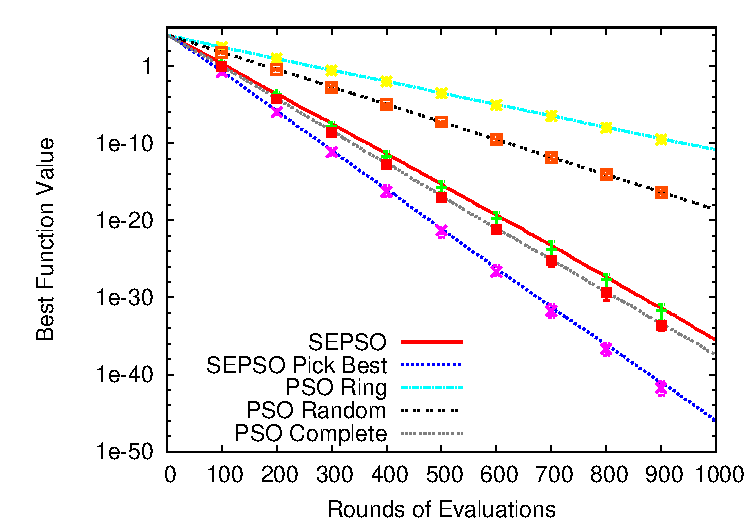
\includegraphics[width=.8\columnwidth]{sphere}
  \caption{Function Sphere with a swarm that uses 240 processors per time step.
  Recall that at each time step all processors evaluate the function once.
  SEPSO uses the Random topology.}
  \label{fig:basic-sphere}
\end{figure}

When we introduce Pick Best, we see more impressive results.  As can be seen in
\fig{sphere-pickbest}, where SEPSO did not manage to perform as well as Na\"ive
Complete, Pick Best handily outperforms it with the same number of processors.

\begin{figure}
  \centering
  \includegraphics[width=.8\columnwidth]{sphere2}
  \caption{Function Sphere with a swarm that uses 240 processors per time step,
  comparing Pick Best with previous results.  All speculative algorithms use
  the Random topology.}
  \label{fig:sphere-pickbest}
\end{figure}

Still more impressive with Sphere are the results of pruning and speculating
several iterations ahead.  Pick Best Pruned outperforms Pick Best, and Many
Iterations by far outperforms every other algorithm on this function.  Many
Iterations on average finds values that are more than 40 orders of magnitude
better than Na\"ive using the same number of processors.  This is shown in
\fig{sphere-manyiters}.  Social Promotion Pruned performed comparably with
SEPSO, and we do not clutter the graph with a line for it.

\begin{figure}
  \centering
  \includegraphics[width=.8\columnwidth]{sphere3}
  \caption{Function Sphere with a swarm that uses 240 processors per time step,
  comparing speculating several iterations ahead with previous results.  All
  speculative algorithms use the Random topology.}
  \label{fig:sphere-manyiters}
\end{figure}

\subsection{Schwefel 2.21}

Schwefel 2.21 is a function similar to Sphere, but Schwefel 2.21 is benefited
more by larger swarms than Sphere is.  Thus our speculative algorithms often
fail to perform as well as Na\"ive because of their smaller swarm size.  In
comparing SEPSO to Na\"ive in \fig{schwefel1}, we can see that SEPSO fails to
perform any better than Na\"ive with a Random topology, and it is by far
outperformed by Na\"ive with a Complete topology.

\begin{figure}
  \centering
  \includegraphics[width=.8\columnwidth]{schwefel1}
  \caption{Function Schwefel with a swarm that uses 240 processors per time
  step.  Recall that at each time step all processors evaluate the function
  once.  SEPSO uses a Random topology.}
  \label{fig:schwefel1}
\end{figure}

As can be seen in \fig{schwefel2}, almost all of the speculative algorithms
perform worse than Na\"ive Complete, with Many Iterations performing comparably
to Na\"ive.  However, one of the speculative algorithms did perform better than
Na\"ive: Pick Best Pruned.  It seems that the larger swarm size available
because of pruning was the cause of the improved performance.  Note that Many
Iterations was initially performing comparably with Pick Best Pruned, but with
more iterations gradually degraded in performance to the level of Na\"ive
Complete.  It is likely that Many Iterations got caught in local optima, and
with more processors would have maintained better performance.

\begin{figure}
  \centering
  \includegraphics[width=.8\columnwidth]{schwefel2}
  \caption{Function Schwefel with a swarm that uses 240 processors per time
  step, comparing all speculative algorithms.  All speculative algorithms use
  the Random topology.}
  \label{fig:schwefel2}
\end{figure}

\subsection{Griewank}

Next we look at the function Griewank.  It is generally recommended to use the
Ring topology when optimizing the Griewank function, as Complete is prone to
premature convergence on a local
optimum~\citep{bratton-2007-defining-a-standard-for-pso}.  Griewank has a
global optimum with a value of 0, and sometimes the swarm finds the optimum and
sometimes it does not.  Instead of showing average function value at each
iteration, a more informative plot for Griewank shows the percent of runs that
have found the global optimum by each iteration.  We ran 50 trials of each
experiment with Griewank, so that the curves are more smooth.  We show results
in \fig{basic-griewank1} for swarms of size 30 and 240 using the Ring topology.
One can see in the figure that the SEPSO approach finds the optimum faster than
the Na\"ive approach.  However, because the swarm size is so small, SEPSO gets
stuck a little less than half of the time.

\begin{figure}
  \centering
  \includegraphics[width=.8\columnwidth]{griewank1}
  \caption{Function Griewank with a swarm that uses 240 processors per time
  step.  Recall that at each time step all processors evaluate the function
  once.  Instead of showing average function value, we show the percentage of
  runs that have found the global optimum by each iteration.  All algorithms
  use the Ring topology.}
  \label{fig:basic-griewank1}
\end{figure}

Because the speculative algorithm got stuck with such a small swarm size, we
ran a set of experiments on Griewank with 800 processors, giving swarms of size
100 and 800 instead of 30 and 240.  \fig{basic-griewank2} shows the results.
\fig{basic-griewank2} is very similar to \fig{basic-griewank1}, except that
speculative evaluation finds the global optimum essentially 100\% of the time.
Thus with a few more processors, our algorithm finds the optimum on average
twice as fast as the Na\"ive approach without a significant loss of accuracy.

\begin{figure}
  \centering
  \includegraphics[width=.8\columnwidth]{griewank2}
  \caption{Function Griewank with a swarm that uses 800 processors per time
  step.  All algorithms use the Ring topology.}
  \label{fig:basic-griewank2}
\end{figure}

In order to show the premature convergence properties of the various approaches
we have presented, we will show results first with swarms using 240 processors,
where these are more visible.  Then we will present an overall result for 800
processors, where using our techniques is generally more successful.

When we look at the performance of our Pick Best approach, a less intuitive
result occurs with Griewank than with Sphere.  Because Sphere needs very little
exploration, the seemingly greedy approach of Pick Best does very well.  But it
also greatly improves performance on Griewank.  In \fig{griewank-pickbest} we
see that Pick Best improves accuracy over SEPSO by 20\%, while at the same time
finding the optimum over 100 rounds of evaluation sooner on average.  It seems
that while Pick Best is locally greedy, there is enough exploration in the
seven speculative evaluations to overcome the inherent greediness of the
approach.

\begin{figure}
  \centering
  \includegraphics[width=.8\columnwidth]{griewank3}
  \caption{Function Griewank with a swarm that uses 240 processors per time
  step, comparing Pick Best with previous results.  All algorithms use the Ring
  topology.}
  \label{fig:griewank-pickbest}
\end{figure}

When we introduce pruning, our intuition about Pick Best turns out to be more
correct.  While adding 50 more particles to the swarm (as pruning allows us to
have 80 particles with 240 processors instead of only 30), Pick Best with
pruning still gets stuck just as often as the original Pick Best.  However,
Social Promotion does well with pruning; it increases the success rate to close
to 100\%, while still finding the optimum on average much faster than the
original PSO.  These results are shown in \fig{griewank-pruned}.

\begin{figure}
  \centering
  \includegraphics[width=.8\columnwidth]{griewank4}
  \caption{Function Griewank with a swarm that uses 240 processors per time
  step, comparing pruning with previous results.  All algorithms use the Ring
  topology.}
  \label{fig:griewank-pruned}
\end{figure}

With Griewank, the premature convergence problems inherent in picking the best
child are exacerbated when speculating several iterations ahead.  When Many
Iterations finds the optimum, it finds it quicker than any other method we
tried, on average four times faster than Na\"ive.  However, it also gets stuck
and fails to find the optimum more than any other method.  The results are
shown in \fig{griewank-manyiters}.   \fig{griewank-manyiters} is also
interesting in that it highlights the trade-off between accuracy and speed in
the various approaches at this swarm size.  The faster the approach finds the
optimum, the less likely it is to be successful.

\begin{figure}
  \centering
  \includegraphics[width=.8\columnwidth]{griewank5}
  \caption{Function Griewank with a swarm that uses 240 processors per time
  step, comparing speculating several iterations ahead with previous results.
  All algorithms use the Ring topology.}
  \label{fig:griewank-manyiters}
\end{figure}

Now that we have seen the effect that the various approaches have on speed of
convergence and success rates, we show a result for using 800 processors, where
most of the approaches have a 100\% success rate.  In this case, the best
algorithm to use is the one which finds the optimum the fastest.  As can be
seen in \fig{griewank-800}, with 800 processors the best choice is Pick Best,
which finds the optimum on average three times as fast as standard PSO.  With
just a few more processors, however, Many Iterations would likely have a 100\%
success rate as well, making it the preferred choice.

\begin{figure}
  \centering
  \includegraphics[width=.8\columnwidth]{griewank6}
  \caption{Function Griewank with a swarm that uses 800 processors per time
  step.  All algorithms use the Ring topology.}
  \label{fig:griewank-800}
\end{figure}

\subsection{Bohachevsky}

Bohachevsky is a unimodal function best optimized with a Complete swarm.  It is
similar to Griewank in that there is a global optimum with a value of 0, and
the swarm sometimes finds it and sometimes does not.  Since we have already
demonstrated the convergence properties of the various algorithms with
Griewank, for Bohachevsky we merely present the best results.  In
\fig{bohachevsky} we can see that all of the speculative approaches found the
optimum much quicker than Na\"ive with a Random topology.  However, SEPSO was
slower than Na\"ive Complete and got stuck around 15\% of the time.  Pick Best,
Pick Best Pruned, and Many Iterations all outperformed Na\"ive Complete, with
Many Iterations finding the optimum about twice as fast.

\begin{figure}
  \centering
  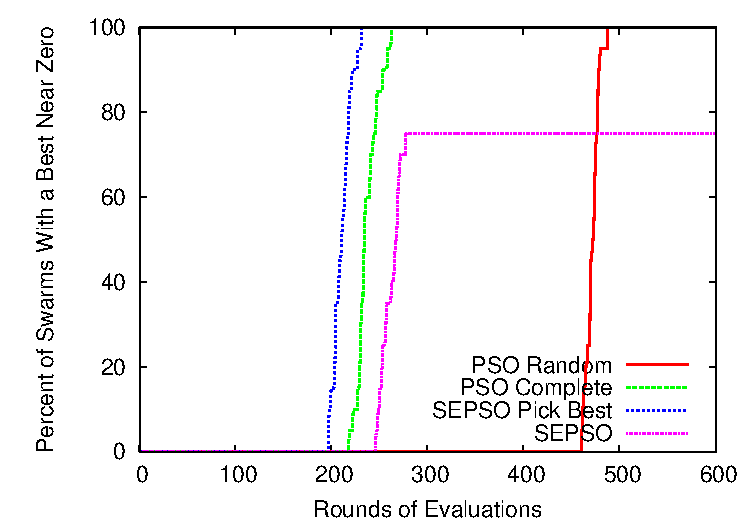
\includegraphics[width=.8\columnwidth]{bohachevsky}
  \caption{Function Bohachevsky with a swarm that uses 800 processors per time
  step.  Recall that at each time step all processors evaluate the function
  once.  All of the speculative algorithms use the Random topology.}
  \label{fig:bohachevsky}
\end{figure}

\section{Conclusions}
\label{sec:conclusion}

We have described a new technique for using processors in parallel PSO to
improve the performance of the algorithm.  To our knowledge, this is the first
time extra processors have been used to do anything in PSO besides increase the
swarm size.  In an increasingly parallel world, such advancements will prove to
be crucial to the continued effectiveness of PSO.

We have detailed how to perform speculative evaluation in PSO in several
different parallel frameworks.  Using this methodology, the behavior of the
original PSO algorithm can either be exactly reproduced, two iterations at a
time, or the behavior can be modified in order to improve performance.  While
exactly reproducing PSO often uses too many extra processors to be useful, when
we allow ourselves some freedom with the algorithm we see great improvements
over previous methods.  We have shown results that conclusively demonstrate the
superiority of our techniques for several functions over na\"ively adding
particles to the swarm when extra processors are available.

What we have presented is not a new algorithm or a variant of PSO, and thus we
did not compare our methods against the state of the art PSO variants.  We
presented a new parallelization technique, so we compared parallelization
strategies on the same algorithm, the original PSO.

We have given five different possible approaches to speculative evaluation,
each of which has different properties.  These approaches perform differently
on different functions and at different swarm sizes, as would be expected by
the No Free Lunch Theorem~\citep{wolpert-1997-nfl-for-optimization}.  We have
given a brief evaluation of the premature convergence properties of these
methods on deceptive functions.  Though there is no one approach that performs
best across all functions at the swarm sizes we used, for all but one of the
functions we looked at \emph{some} kind of speculative evaluation outperforms
standard PSO, often dramatically.  It also appears to us that once enough
processors are available, by far the best approach is to speculate as many
iterations ahead as processors allow.

Though our methods show great improvements on some functions, they do not work
for all functions at the swarm sizes we were able to test with.  As is commonly
known, in PSO there is a trade-off between exploration and exploitation.  Some
functions need only minimal exploration, and some never seem to have enough.
Increasing the swarm size is a natural way to increase exploration in a
parallel environment.  However, once ``enough'' exploration has been reached
for any particular function, adding additional particles adds only incremental
benefits.  A better use of the additional processors, as we have shown, is to
perform some amount of speculative evaluation.

Sphere is a function for which only a very small amount of exploration needs to
be done, and our speculative methods show improvements on Sphere of over 40
orders of magnitude.  Our methods work very well on these functions.

Rastrigin, on the other hand, is a function for which increasing the swarm size
up to 4000 particles still shows improvements in the performance of the
algorithm.  With such functions, the smaller swarm size required by speculative
evaluation does not produce enough exploration to perform better than standard
PSO at the swarm sizes we were able to experiment with.

Griewank is a function in between Sphere and Rastrigin (as are Bohachevsky and
Schwefel 2.21).  It is highly deceptive and is prone to premature convergence,
but by adding particles to the swarm a point is reached where ``enough''
exploration is done, and the algorithm finds the optimum essentially all of the
time.  For such functions, the best approach seems to be to increase the swarm
size until ``enough'' exploration is reached, then use extra processors to
perform speculative evaluation and increase the number of iterations performed.
Sphere and Rastrigin can be thought of as special cases of these types of
functions; Sphere simply needs a very small swarm size to produce ``enough''
exploration, and Rastrigin requires a very large swarm.  We expect that for all
functions there is a swarm size for which additional particles are less useful
than additional iterations.

Large parallel clusters are often required to successfully optimize practical
modern problems.  To properly use PSO with such clusters, a balance needs to be
made between using processors to increase the swarm size and using them to
increase the speed of the algorithm.  This work is a first step in that
direction.

\section{Future Work}
\label{sec:future}

We have presented a new paradigm for parallelizing the particle swarm
optimization algorithm, focusing on PSO itself and not all of its variants.  It
remains as future work to apply speculative approaches to recent and popular
PSO variants, such as the Fully Informed Particle
Swarm~\citep{mendes-2004-fully-informed-particle-swarm}.  While our methods
will not always be immediately applicable to every variant, we are confident
that some kind of speculative approach will be beneficial to the
parallelization of all forms of PSO, especially as the number of processors
used gets into the thousands.

We mentioned related work showing that increasing the swarm size throughout the
course of the algorithm could provide improved performance over a fixed swarm
size in serial PSO~\citep{montes-de-oca-2010-incremental-social-learning-pso}.
If this method were extended to parallel PSO, most processors would be idle in
the first few iterations, while more would be utilized at the end.  During
iterations where there are many un-utilized processors, a natural use of them
would be speculative evaluation, performing two or more of those iterations at
a time.  Thus our methods have the potential to further improve the parallel
performance of recently proposed variations of PSO.

We have speculated that our Pick Best method simply draws a number of samples
from the next iteration of the sampling distribution of PSO and keeps one of
them.  It would then be expected that the sampling distribution of that method
is very similar to the distribution of the original
PSO~\citep{poli-2008-sampling-distribution-of-pso}.  This remains to be proven,
or even demonstrated empirically.

We gave a passing glance to some very interesting statistical characteristics
of PSO.  Our motivation was to use the statistics to improve our speculative
algorithm, but it seems there are some nuggets in the numbers that could be
used to improve our understanding of the behavior of PSO in general, and what
role a topology plays.  A potentially very fruitful avenue of future work would
be to further analyze the branch statistics in PSO across many functions and
topologies, categorizing both the topologies and the functions and discovering
what it is that makes certain topologies work well with certain functions.
There are also some particles that seem to drive the swarm and others that are
stagnant almost the entire time.  Such information could be used in a
TRIBES-like fashion~\citep{clerc-2003-tribes} to determine which particles
should be removed from the swarm, perhaps starting them close to
well-performing particles.

We turned what used to be a very simple algorithm with only one major parameter
to tweak (the topology) into a convoluted mess with countless possibilities for
speculative evaluations.  Perhaps future research will be able to narrow down
the endless possibilities into the few best ones, making the algorithm simple
again.  We have presented some small amount of exploration of the possible
alternatives, but our discussion is by no means exhaustive or conclusive.

Our methods for determining which speculative evaluations to perform were
independent of the particle; all particles performed the same number and type
of evaluations.  Another way to allocate speculative evaluations is to somehow
use the performance of each particle to determine how many and which extra
evaluations it can have.  We imagine that the benefits of intelligently and
dynamically deciding which particles get extra evaluations could produce very
good results.  Future work could explore the use of a centralized allocator for
extra processors or ideas in the multi-robot task allocation literature, such
as auctions, to better assign processors to particles for speculative
evaluations.  While such methods involve extra communication, with long-running
function evaluations the extra overhead of intelligently allocating resources
would likely be negligible.

A technique similar to ours has been previously used to parallelize simulated
annealing~\citep{witte-1991-parallel-simulated-annealing-speculative}.  Any
other optimization algorithm that only depends on current sampling positions
when computing the next position to sample can be parallelized with this
technique.  In particular, genetic algorithms produce future generations by
combining individuals from the current generation.  With a large population
size there would be an unwieldy amount of possible future individuals, but the
potential exists to modify the algorithm to use some kind of speculative
evaluation.  A related but quite distinct technique for reducing computation in
evolutionary algorithms was proposed
in~\citep{poli-2006-backward-chaining-evolutionary-algorithms}.

\section*{Appendix---Alternate form of message passing}

Here we describe a method that requires only one round of communication for
each pair of iterations, which happens at step 5 of \alg{centralized}.  Many
more messages are needed, but that is sometimes more desirable than
synchronizing all of the machines three times.

This second method only requires one round of passing information because
information about both iterations $t$ and $t+1$ is passed at the same time.
Each processor reconstructs from the messages it receives all of the
information that it needs about its neighbors.  Messages are passed directly
after evaluating each particle and its children, so all messages are of the
form of $\nonbest{\p}_t$ or $\nonbest{\s}_{t+1}$.  The first iteration needs to
be treated specially, so each particle can produce its initial set of
speculative children---neighbors need only pass their initial position.  This
kind of message passing necessitates the careful use of random seeds, so that
when each processor computes the motion equations for its neighbors it gets the
same results as its neighboring processors.

With the results of evaluating $\noeval{\p}_t$ and $\noeval{\sset}_{t+1}$,
along with all of the required messages from neighboring particles, the goal is
to produce $\p_{t+1}$ and output $\noeval{\p}_{t+2}$ and $\noeval{\sset}_{t+3}$
ready to be evaluated for the next iteration.  We first focus on the messages
needed to produce $\p_{t+1}$.

Upon evaluation, $\noeval{\p}_t$ becomes $\nonbest{\p}_t$, needing only to get
its neighborhood best information from its neighbors.  All of its neighbors,
then, must send it a message, so that from their updated personal best at
iteration $t$ the particle becomes $\p_t$.  The work done with the messages
received thus far is just as in regular PSO, and is graphically depicted in 
\fig{messages1}.

\begin{figure}
  \centering
  \psfrag{pt-n}[C][C]{$\nonbest{\p}_{t}$}
  \psfrag{nt-n}[C][C]{$\nonbest{\nset}_{t}$}
  \psfrag{pt}[C][C]{$\p_{t}$}
  \includegraphics[width=.15\columnwidth]{messages1}
  \caption{The production of $\p_{t}$ from the original particle
  $\nonbest{\p}_{t}$ and the messages $\nonbest{\nset}_{t}$.}
  \label{fig:messages1}
\end{figure}

With $\p_t$ we can select the correct speculative child as described above and
produce $\nonbest{\p}_{t+1}$.  Again we show the use of messages thus far
graphically, in \fig{messages2}.  

\begin{figure}
  \centering
  \psfrag{pt-n}[C][C]{$\nonbest{\p}_{t}$}
  \psfrag{nt-n}[C][C]{$\nonbest{\nset}_{t}$}
  \psfrag{pt}[C][C]{$\p_{t}$}
  \psfrag{pt1-n}[C][C]{$\nonbest{\p}_{t+1}$}
  \psfrag{st1-n}[C][C]{$\nonbest{\sset}_{t+1}$}
  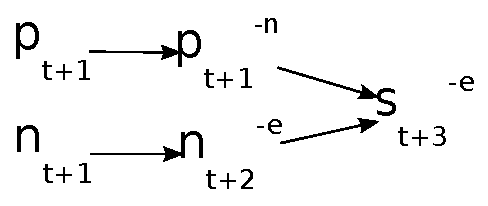
\includegraphics[width=.25\columnwidth]{messages2}
  \caption{The production of $\nonbest{\p}_{t+1}$ from the original particle 
  $\nonbest{\p}_{t}$, messages $\nonbest{\nset}_{t}$ and
  $\nonbest{\sset}_{t+1}$, and intermediate particles.}
  \label{fig:messages2}
\end{figure}

We then need the set of neighbors to $\nonbest{\p}_{t+1}$,
$\nonbest{\nset}_{t+1}$, so we can update $\nonbest{\p}_{t+1}$'s neighborhood
best.  To produce each neighbor $\nonbest{\n}_{t+1}$, we need the same
information for the neighboring particle that we needed to produce the original
particle, $\nonbest{\p}_{t+1}$; we need the original neighbor particle, its
speculative children, and its neighbors.  With that information, the set
$\nonbest{\nset}_{t+1}$ can be obtained by following the same process used to
obtain $\nonbest{\p}_{t+1}$.  We graphically show the messages needed to
produce $\nonbest{\nset}_{t+1}$ in \fig{messages3}.  Note that it looks
identical to \fig{messages2}, just with different sets of particles.

\begin{figure}
  \centering
  \psfrag{nt-n}[C][C]{$\nonbest{\nset}_{t}$}
  \psfrag{nnt-n}[C][C]{$\nonbest{\nnset}_{t}$}
  \psfrag{nt}[C][C]{$\nset_{t}$}
  \psfrag{nt1-n}[C][C]{$\nonbest{\nset}_{t+1}$}
  \psfrag{nst1-n}[C][C]{$\nonbest{\nsset}_{t+1}$}
  \includegraphics[width=.3\columnwidth]{messages3}
  \caption{The production of each $\nonbest{\n}_{t+1}$ from the original
  particle $\nonbest{\n}_{t}$, messages $\nonbest{\nnset}_{t}$ and
  $\nonbest{\nsset}_{t+1}$, and intermediate particles.  $\nnset$ is the set of
  neighbors for each particle $\n$, and $\nsset$ is the set of $\n$'s
  speculative children.  Note the similarity between this and \fig{messages2}.}
  \label{fig:messages3}
\end{figure}

With $\nonbest{\nset}_{t+1}$ and $\nonbest{\p}_{t+1}$, we can produce
$\p_{t+1}$.  This is shown in \fig{messages4}.  Note that we just combined
Figures~\ref{fig:messages2}~and~\ref{fig:messages3}, putting them together
to make $\p_{t+1}$, as all the particle needs is its neighborhood best to be
updated.

\begin{figure}
  \centering
  \psfrag{pt-n}[C][C]{$\nonbest{\p}_{t}$}
  \psfrag{nt-n}[C][C]{$\nonbest{\nset}_{t}$}
  \psfrag{pt}[C][C]{$\p_{t}$}
  \psfrag{pt1-n}[C][C]{$\nonbest{\p}_{t+1}$}
  \psfrag{st1-n}[C][C]{$\nonbest{\sset}_{t+1}$}
  \psfrag{nt-n}[C][C]{$\nonbest{\nset}_{t}$}
  \psfrag{nnt-n}[C][C]{$\nonbest{\nnset}_{t}$}
  \psfrag{nt}[C][C]{$\nset_{t}$}
  \psfrag{nt1-n}[C][C]{$\nonbest{\nset}_{t+1}$}
  \psfrag{nst1-n}[C][C]{$\nonbest{\nsset}_{t+1}$}
  \psfrag{pt1}[C][C]{$\p_{t+1}$}
  \includegraphics[width=.4\columnwidth]{messages4}
  \caption{The production of $\p_{t+1}$ from the original particle 
  $\nonbest{\p}_{t}$, messages $\nonbest{\nset}_{t}$, $\nonbest{\sset}_{t+1}$,
  $\nonbest{\nnset}_{t}$, and $\nonbest{\nsset}_{t+1}$, and intermediate
  particles.  Note that this is just a combination of \fig{messages2} and
  \fig{messages3}.}
  \label{fig:messages4}
\end{figure}

In order to get $\p_{t+1}$, then, a particle needs to receive messages from its
neighbors, its neighbors' neighbors, its speculative children, and its
neighbors' speculative children.  The particle $\p_{t+1}$ can be passed to some
central machine to track the progress of the algorithm, and it can be moved to
$\noeval{\p}_{t+2}$ in order to start the next iteration.

The next goal is to produce the set $\noeval{\sset}_{t+3}$.  As described
above, the necessary components to produce $\noeval{\sset}_{t+3}$ are
$\noeval{\p}_{t+2}$ and the neighbors of $\noeval{\p}_{t+2}$,
$\noeval{\nset}_{t+2}$.  We already have $\noeval{\p}_{t+2}$, so what remains
is to produce $\noeval{\nset}_{t+2}$.  It is sufficient to obtain
$\nset_{t+1}$, as each neighbor particle $\n_{t+1}$ can be moved with the
motion equations to $\noeval{\n}_{t+2}$.

We have already described how to use a set of messages to obtain $\p_{t+1}$.
The process is exactly the same to produce each $\n_{t+1}$, requiring the same
messages, only for the neighbor particles instead of the particle itself.
\fig{messages5} shows graphically how $\noeval{\sset}_{t+3}$ is produced.

\begin{figure}
  \centering
  \psfrag{pt1}[C][C]{$\p_{t+1}$}
  \psfrag{nt1}[C][C]{$\nset_{t+1}$}
  \psfrag{nt2-e}[C][C]{$\noeval{\nset}_{t+2}$}
  \psfrag{pt2-e}[C][C]{$\noeval{\p}_{t+2}$}
  \psfrag{st3-e}[C][C]{$\noeval{\sset}_{t+3}$}
  \includegraphics[width=.25\columnwidth]{messages5}
  \caption{The production of $\noeval{\p}_{t+2}$ and $\noeval{\sset}_{t+3}$
  from $\p_{t+1}$ and $\n_{t+1}$, each of which are produced as in
  \fig{messages4}.}
  \label{fig:messages5}
\end{figure}

Having obtained both $\noeval{\p}_{t+2}$ and $\noeval{\sset}_{t+3}$ from the
messages received, the algorithm then moves to the evaluation phase, and the
process repeats itself.  The particles are evaluated, send their messages, and
produce the next set of particles to be evaluated from the messages received.

To perform the entire process, at each message passing round a particle must
receive messages from its neighbors, its neighbors' neighbors, its neighbors'
neighbors' neighbors, its speculative children, its neighbors' speculative
children, and its neighbors' neighbors' speculative children.  With the Ring
topology, that looks like more messages than it really is, as many of the
neighbors' neighbors are duplicates.  With the Random topology, however, the
list of necessary messages could be rather large.  

One more issue arises when dealing with dynamic topologies.  With neighbors
changing each iteration, messages that processors pass to their neighbors need
to be sent to the correct neighbors for each iteration.  A particle cannot
simply send messages to its neighbors' neighbors' neighbors---it needs to send
messages to its iteration $t$ neighbors' iteration $t+1$ neighbors, and so on.
For every neighbor outward information is sent, the iteration also needs to be
incremented, as information about neighbors' neighbors is used during iteration
$t+1$, and information about neighbors' neighbors' neighbors is used to
reconstruct information about iteration $t+2$.  Also, this method of message
passing again requires the use of random seeds if the topology is random, so
that each processor computes the same neighbors for a particle as all other
processors.

This may seem like an inordinate amount of work, and with some distributed PSO
frameworks it is.  However, other parallel frameworks necessitate this type of
message passing, so we have described how speculative evaluation can be
performed in those circumstances.


\bibliographystyle{apa-good}
\bibliography{%
../../../bib/aml/bib,%
../../../bib/nfl/bib,%
../../../bib/optimization/bib,%
../../../bib/parallel/bib,%
../../../bib/pso/general/bib,%
../../../bib/pso/parallel/bib,%
../../../bib/pso/fips/bib,%
../../../bib/pso/topology/bib,%
../../../bib/sim-anneal/parallel/bib,%
../../../bib/ga/bib}

\end{document}
